\chapter{Interfaces}

\subsection{AHB-Lite Interface}

The AHB-Lite interface is a regular AHB-Lite slave port. All signals are
supported. See the
\emph{\href{https://www.arm.com/products/system-ip/amba-specifications}{AMBA
3 AHB-Lite Specification}} for a complete description of the signals.

\begin{longtable}[c]{@{\extracolsep{\fill}}cccl@{}}	
		\toprule 
		\textbf{Port} & \textbf{Size} & \textbf{Direction} & \textbf{Description}\\
		\midrule
		\endhead 
		\texttt{HRESETn} & 1 & Input & Asynchronous active low reset\\
		\texttt{HCLK} & 1 & Input & Clock Input\\
		\texttt{HSEL} & 1 & Input & Bus Select\\
		\texttt{HTRANS} & 2 & Input & Transfer Type\\
		\texttt{HADDR} & \texttt{HADDR\_SIZE} & Input & Address Bus\\
		\texttt{HWDATA} & \texttt{HDATA\_SIZE} & Input & Write Data Bus\\
		\texttt{HRDATA} & \texttt{HDATA\_SIZE} & Output & Read Data Bus\\
		\texttt{HWRITE} & 1 & Input & Write Select\\
		\texttt{HSIZE} & 3 & Input & Transfer Size\\
		\texttt{HBURST} & 3 & Input & Transfer Burst Size\\
		\texttt{HPROT} & 4 & Input & Transfer Protection Level\\
		\texttt{HREADYOUT} & 1 & Output & Transfer Ready Output\\
		\texttt{HREADY} & 1 & Input & Transfer Ready Input\\
		\texttt{HRESP} & 1 & Output & Transfer Response\\
		\bottomrule 	
	\caption{PLIC Interface Signals}
	\label{tab:AHBIF}
\end{longtable}

\subsubsection{HRESETn}

When the active low asynchronous \texttt{HRESETn} input is asserted
(`0'), the interface is put into its initial reset state.

\subsubsection{HCLK}

\texttt{HCLK} is the interface system clock. All internal logic for the
AHB-Lite interface operates at the rising edge of this system clock and
AHB bus timings are related to the rising edge of \texttt{HCLK}.

\subsubsection{HSEL}

The AHB-Lite interface only responds to other signals on its bus -- with
the exception of the global asynchronous reset signal \texttt{HRESETn}
-- when \texttt{HSEL} is asserted (`1'). When \texttt{HSEL} is negated
(`0') the interface considers the bus \texttt{IDLE}.

\subsubsection{HTRANS}

HTRANS indicates the type of the current transfer as shown in Table \ref{tab:HTRANS}

\begin{longtable}[c]{@{\extracolsep{\fill}}ccp{7cm}}	
		\toprule 
		\textbf{HTRANS} & \textbf{Type} & \textbf{Description}\\
		\midrule
		\endhead 
		00 & \texttt{IDLE} & No transfer required\\
		01 & \texttt{BUSY} & Connected master is not ready to accept data, but intents to continue the current burst.\\
		10 & \texttt{NONSEQ} & First transfer of a burst or a single transfer\\
		11 & \texttt{SEQ} & Remaining transfers of a burst\\
		\bottomrule 	
	\caption{HTRANS Signal Types}
	\label{tab:HTRANS}
\end{longtable}

\subsubsection{HADDR}

\texttt{HADDR} is the address bus. Its size is determined by the
\texttt{HADDR\_SIZE} parameter and is driven to the connected
peripheral.

\subsubsection{HWDATA}

\texttt{HWDATA} is the write data bus. Its size is determined by the
\texttt{HDATA\_SIZE} parameter and is driven to the connected
peripheral.

\subsubsection{HRDATA}

\texttt{HRDATA} is the read data bus. Its size is determined by the
\texttt{HDATA\_SIZE} parameter and is sourced by the connected
peripheral.

\subsubsection{HWRITE}

\texttt{HWRITE} is the read/write signal. \texttt{HWRITE} asserted (`1')
indicates a write transfer.

\subsubsection{HSIZE}

\texttt{HSIZE} indicates the size of the current transfer as shown in table \ref{tab:HSIZE}:

\begin{longtable}[c]{@{\extracolsep{\fill}}ccl}	
		\toprule 
		\textbf{HSIZE} & \textbf{Size} & \textbf{Description}\\
		\midrule
		\endhead 
		000 & 8 bit & Byte\\
		001 & 16 bit & Half Word\\
		010 & 32 bit & Word\\
		011 & 64 bits & Double Word\\
		100 & 128 bit &\\
		101 & 256 bit &\\
		110 & 512 bit &\\
		111 & 1024 bit &\\
		\bottomrule 	
	\caption{HSIZE Values}
	\label{tab:HSIZE}
\end{longtable}

\subsubsection{HBURST}

HBURST indicates the transaction burst type -- a single transfer or part
of a burst.

\begin{longtable}[c]{@{\extracolsep{\fill}}ccl}	
		\toprule 
		\textbf{HBURST} & \textbf{Type} & \textbf{Description}\\
		\midrule
		\endhead 
		000 & \texttt{SINGLE} & Single access**\\
		001 & \texttt{INCR} & Continuous incremental burst\\
		010 & \texttt{WRAP4} & 4-beat wrapping burst\\
		011 & \texttt{INCR4} & 4-beat incrementing burst\\
		100 & \texttt{WRAP8} & 8-beat wrapping burst\\
		101 & \texttt{INCR8} & 8-beat incrementing burst\\
		110 & \texttt{WRAP16} & 16-beat wrapping burst\\
		111 & \texttt{INCR16} & 16-beat incrementing burst\\
		\bottomrule 	
	\caption{HBURST Types}
	\label{tab:HBURST}
\end{longtable}

\subsubsection{HPROT}

The \texttt{HPROT} signals provide additional information about the bus
transfer and are intended to implement a level of protection.

\begin{longtable}[c]{@{}lccl}	
		\toprule 
		& \textbf{Bit\#} & \textbf{Value} & \textbf{Description}\\
		\midrule
		\endhead 
		& 3 & 1 & Cacheable region addressed\\
		& & 0 & Non-cacheable region addressed\\
		& 2 & 1 & Bufferable\\
		& 0 & Non-bufferable\\
		& 1 & 1 & Privileged Access\\
		& & 0 & User Access\\
		& 0 & 1 & Data Access\\
		& & 0 & Opcode fetch\\
		\bottomrule 	
	\caption{HPROT Indicators}
	\label{tab:HPROT}
\end{longtable}

\subsubsection{HREADYOUT}

\texttt{HREADYOUT} indicates that the current transfer has finished.
Note, for the AHB-Lite PLIC this signal is constantly asserted as the
core is always ready for data access.

\subsubsection{HREADY}

\texttt{HREADY} indicates whether or not the addressed peripheral is
ready to transfer data. When \texttt{HREADY} is negated (`0') the
peripheral is not ready, forcing wait states. When \texttt{HREADY} is
asserted (`1') the peripheral is ready and the transfer completed.

\subsubsection{HRESP}

\texttt{HRESP} is the instruction transfer response and indicates OKAY
(`0') or ERROR (`1').


\section{PLIC Interface} 

\missingfigure{Test} \todo[author=SPH, color=red]{Add PLIC Interface Intro}

\begin{longtable}[c]{@{\extracolsep{\fill}}lccl@{\extracolsep{\fill}}}	
	\toprule
	\textbf{Port} & \textbf{Size} & \textbf{Direction} & \textbf{Description}\\
	\midrule 
	\endhead
	\texttt{SRC} & \texttt{SOURCES} & Input & Interrupt Sources\\
	\texttt{IRQ} & \texttt{TARGETS} & Output & Interrupt Requests \\
	\bottomrule 	
	\caption{PLIC Interface Signals} 
	\label{tab:PLICIF2}
\end{longtable}

Note: Width of PLIC interface buses are defined by
\protect\hyperlink{core-parameters}{Core Parameters}.

\subsection{SRC}

Interrupt sources connect to the \texttt{SRC{[}SOURCES-1..0{]}} input of
the PLIC module. The width of this interface is defined by the
\protect\hyperlink{SOURCES}{\texttt{SOURCES}} parameter.

\subsection{IRQ}

Interrupt targets are sourced by the \texttt{IRQ{[}TARGETS-1..0{]}}
output of the PLIC module. The width of this interface is defined by the
\protect\hyperlink{TARGETS}{\texttt{TARGETS}} parameter.

\section{Register Interface}

The following registers are user accessible in the PLIC module:

\begin{longtable}[c]{@{\extracolsep{\fill}}ccccp{5cm}@{\extracolsep{\fill}}}	
	\toprule 
	\textbf{Register} & \textbf{Registers} & \textbf{Width (bits)} & \textbf{Mode} & \textbf{Function} \\
	\midrule 
	\endhead
	\texttt{CONFIG} & 1 & 64 & RO & Configuration\\
	\texttt{EL} & 1 & \texttt{SOURCES} & RW & Edge/Level Trigger\\
	\texttt{IE} & \texttt{TARGETS} & \texttt{SOURCES} & RW & Interrupt Enable\\
	\texttt{ID} & \texttt{TARGETS} & clog\textsubscript{2}(\texttt{SOURCES}) & RW & ID of Highest priority IRQ, \newline Int. Claim (R), \newline Int. Complete (W)\\
	\texttt{PRIORITY} & \texttt{SOURCES} & clog\textsubscript{2}(\texttt{PRIORITIES}) & RW & Priority Level\\
	\texttt{THRESHOLD} & \texttt{TARGETS} & clog\textsubscript{2}(\texttt{PRIORITIES}) & RW & Priority Threshold \\
	\bottomrule 	

\caption{PLIC Register Interface}
\label{tab:REGIF2}
\end{longtable}

Note: clog\textsubscript{2}() refers to the System Verilog function by
the same name, defined as:

\begin{quote}
\emph{The system function \$clog2 shall return the ceiling of the log
base 2 of the argument (the log rounded up to an integer value). The
argument can be an integer or an arbitrary sized vector value. The
argument shall be treated as an unsigned value, and an argument value of
0 shall produce a result of 0.}
\end{quote}

\subsection{Register Descriptions}

\subsubsection{CONFIG}

The \texttt{CONFIG} register is a Read-Only register that enables a
software routine to determine the hardware configuration of the PLIC
module.

When enabled via the \texttt{HAS\_CONFIG\_REG} hardware parameter, the
\texttt{CONFIG} register returns a 64 bit value constructed as follows:

\todo[author=SPH, color=red]{Fix diagram Font}

\begin{figure}[h] 
	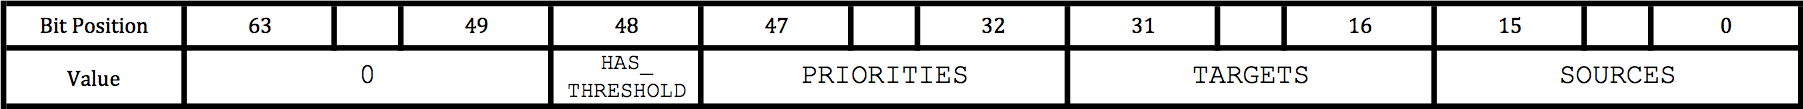
\includegraphics[width=\linewidth]{img/CONFIG.png} 
	\caption[Configuration Register]{Configuration Register}
	\label{fig:configreg}
\end{figure}

The values, \texttt{HAS\_THRESHOLD}, \texttt{PRIORITIES},
\texttt{TARGETS} and \texttt{SOURCES} correspond to the hardware
parameters documented in section 3.1.

\subsubsection{EL}

The \texttt{EL} Read/Write register defines if an interrupt source is
Edge or Level Triggered.

The number of interrupt sources, as defined by the
\protect\hyperlink{SOURCES}{\texttt{SOURCES}} parameter, determines
the width of the \texttt{EL} register. One bit within the register
corresponds to an interrupt source, where a logic high (`1') defines a
rising-edge triggered interrupt and a logic low (`0') defines a level
triggered interrupt.

\subsubsection{IE[]}

The matrix of \texttt{IE[]} Read/Write registers define if an
interrupt source is enabled or disabled for a specific target. When
disabled, any interrupts generated by the source will be ignored by the
PLIC.

The number of targets determines the number of \texttt{IE[]}
registers. The number of interrupt sources, as defined by the
\protect\hyperlink{SOURCES}{\texttt{SOURCES}} parameter, determines the
width of each \texttt{IE[]} register. One bit within the register
corresponds to an individual interrupt source, where a logic high (`1')
defines an interrupt source as enabled and a logic low (`0') as
disabled.

\subsubsection{ID[]}

The \texttt{ID[]} Read/Write register identifies to each target
the ID of the highest priority pending interrupt request.

This register indicates to the target which of potentially multiple
pending interrupts should be serviced rather than relying on this being
resolved by the software Interrupt Service Routine.

When a target reads this register, this also indicates the target has
claimed the interrupt for the defined source and will service then
service the interrupt source.

A target then writes to this register to indicate completion of
servicing the interrupt source. It is the action of writing to this
register which generates the interrupt completion notification -- the
value written will not update the register which continues to identify
the highest priority interrupt source to be serviced.

\subsubsection{PRIORITY[]}

The \texttt{PRIORITY[]} Read/Write registers define the priority level of each interrupt source.

There is one \texttt{PRIORITY[]} register per interrupt source as defined by the \texttt{SOURCES} parameter (see \protect\hyperlink{SOURCES}{\texttt{SOURCES}}), identified as \texttt{PRIORITY[SOURCES-1:0]}. The width of each register is derived from the number of priority levels as defined by the \texttt{PRIORITIES} parameter (see \protect\hyperlink{TARGETS}{\texttt{TARGETS}}).

Interrupt priority increases with larger values of \texttt{PRIORITY}.

\subsubsection{THRESHOLD[]}

Each target may be assigned a priority threshold via the
\texttt{THRESHOLD[]} registers. Only
active interrupts that have a priority strictly greater than the
threshold will cause an interrupt notification to be sent to the target.
A \texttt{THRESHOLD[]} value of 0
means that no interrupts will be masked.

\subsection{Register Address Mapping}

The PLIC supports a wide variety of options and unlimited user-definable
number of both interrupt sources and targets. To configure and control
the PLIC requires a memory-mapped register interface that must be
defined according to the specific implementation.

To ease the development of PLIC based systems, the Roa Logic PLIC
implements a dynamic register interface based on the hardware parameters
set during generation of the implementation, packing multiple bit-fields
into registers where feasible to minimise the required address space.

The following sections describe the calculations performed during
generation of the dynamic register interface so that the user may
determine the registers available and the memory mapping of those
registers for a given implementation.

A spreadsheet in Microsoft Excel format is available to perform these
calculations based on user-defined parameters to show the registers and
memory mapping. Further, simulation of the PLIC will also shows the
registers and memory mapping.

\subsection{Itemising Register Requirements}

The section "\protect\hyperlink{register-interface}{Register Interface}"
provides a summary of the registers required to control and configure
the PLIC. The following is a more detailed summary of those
requirements.

\subsubsection{CONFIG Register:}

The \texttt{CONFIG} register is always 64 bits. For 32 bit
implementations this means 2 physical registers are required, 1 each for
the upper and lower word. For 64 bit implementations a single register
will be implemented.

\subsubsection{EL Registers:}

Each interrupt source requires a single bit in the \texttt{EL} register
to define if the source is level or edge triggered. These bits will be
packed into the minimum number of registers.

The physical number of registers implemented can be calculated as
follows:

\begin{quote}
\texttt{No.\ of\ Registers\ =\ ROUNDUP(SOURCES/HDATA\_SIZE)}
\end{quote}

Example: For a 32 bit system supporting 48 interrupt sources

\begin{verbatim}
No. of Registers = ROUNDUP(SOURCES/HDATA_SIZE)   
                 = ROUNDUP(48/32)
                 = ROUNDUP(1.5)
                 = 2
\end{verbatim}

\subsubsection{IE Registers:}

Interrupt sources may be enabled or disabled per target requiring single
bit per target. These bits will be packed into the fewest registers
possible and the resulting number of registers calculated as follows:

\begin{quote}
\texttt{No.\ of\ Registers\ =\ ROUNDUP(SOURCES/HDATA\_SIZE)*TARGETS}
\end{quote}

Example: For a 32 bit system supporting 48 interrupt sources and 4
targets

\begin{verbatim}
No. of Registers = ROUNDUP(SOURCES/HDATA_SIZE)*TARGETS
                 = ROUNDUP(48/32)*4
                 = ROUNDUP(1.5)*4
                 = 2*4
                 = 8
\end{verbatim}

\subsubsection{ID Registers:}

The \texttt{ID[]} Read/Write
register identifies the ID of the highest priority pending interrupt
request, with one ID register required per target.

\begin{quote}
\texttt{No.\ of\ Registers\ =\ TARGETS}
\end{quote}

\subsubsection{PRIORITY Registers:}

Each interrupt source can be assigned a priority, which is defined as
positive integer. The PLIC parameter \texttt{PRIORITIES} defines the
number of priority levels for a specific implementation, which then
allows a source to be assigned a priority between 1 and
\texttt{PRIORITIES}.

These priority levels are packed into
\texttt{HDATA\_SIZE} bit registers, as fields aligned to
4-bit nibble boundaries

\begin{quote}
\texttt{No.\ of\ Registers\ =\ ROUNDUP(SOURCES/FPR)}
\end{quote}
where:
\indent
\begin{verbatim}
    FPR = FIELDS_PER_REGISTER    
        = HDATA_SIZE/(4*NPP)

    NPP = NIBBLES_PER_PRIORITY
        = ROUNDUP($clog2(PRIORITIES+1)/4)
\end{verbatim}

Example: For a 32 bit system supporting 48 interrupt sources and 8
priority levels

\begin{verbatim}
    NPP = NIBBLES_PER_PRIORITY
        = ROUNDUP($clog2(PRIORITIES+1)/4)
        = ROUNDUP($clog2(8+1)/4)
        = ROUNDUP(4/4)
        = 1

    FPR = FIELDS_PER_REGISTER
        = HDATA_SIZE/(4*NPP)
        = 32/(4*1)
        = 8

    No. of Registers = ROUNDUP(SOURCES/FPR)
                     = ROUNDUP(48/8)
                     = 6
\end{verbatim}

Note: clog\textsubscript{2}() refers to the System Verilog function by
the same name and calculates the number of binary bits required to
represent a given integer.

\subsubsection{THRESHOLD Registers:}

Each target may be assigned a priority threshold and therefore the PLIC
implements 1 register per threshold.

\begin{quote}
\texttt{No.\ of\ Registers\ =\ TARGETS}
\end{quote}

\subsection{Register Address Ordering}

The order of the registers in the memory map is defined as Table \ref{tab:REGMAP}.

\begin{longtable}[h]{@{}cp{4cm}@{}}	
		\toprule 
		\textbf{Order} & \textbf{Registers}\\
		\midrule
		\endhead 
		1 & CONFIG Register(s)\\
		2 & EL Registers\\
		3 & PRIORITY Registers\\
		4 & IE Registers\\
		5 & THRESHOLD Registers\\
		6 & ID Registers\\
		\bottomrule 	
	\caption{Register Address Order}
	\label{tab:REGMAP}
\end{longtable}

Registers are mapped to consecutive addresses based on this order and the
number of registers required. \todo[author=SPH]{Expand register address map section with more details} 

\subsection{Register Address Map Example}

Using the previous example of a 32 bit system supporting 48 interrupt sources, 4 targets and 8 priority levels as shown in Table \ref{tab:REGMAPEX}:

\begin{longtable}[c]{@{}cc@{}}	
		\toprule 
		\textbf{Parameter} & \textbf{Number}\\
		\midrule 
		\endhead
		HDATA\_WIDTH & 32\\
		SOURCES & 48\\
		TARGETS & 4\\
		PRIORITIES & 8\\
		\bottomrule 	
 
	\caption{Register Map Example}
	\label{tab:REGMAPEX}
\end{longtable}

The resulting number of registers is:

\begin{longtable}[c]{@{}cc@{}}	
		\toprule 
		\textbf{Registers} & \textbf{Number}\\
		\midrule 
		\endhead
		CONFIG & 2\\
		EL & 2\\
		PRIORITY & 6\\
		IE & 8\\
		THRESHOLD & 4\\
		ID & 4\\
		\midrule
		\textbf{Total} & \textbf{26}\\
		\bottomrule 	
	\caption{Calculated Registers}
	\label{tab:REGMAPNUM}
\end{longtable}

These registers will be then mapped as follows according to the order
defined in Table \ref{tab:REGMAP}:

\begin{longtable}[c]{ccc}	
		\toprule 
		\textbf{Reg} & \textbf{Parameter} & \textbf{Value}\\
		\midrule 
		\endhead
		\textbf{0} & 0x0 & CONFIG\\
		\textbf{1} & 0x4 & CONFIG\\
		\textbf{2} & 0x8 & EL\\
		\textbf{3} & 0xC & EL\\
		\textbf{4} & 0x10 & PRIORITY\\
		\textbf{5} & 0x14 & PRIORITY\\
		\textbf{6} & 0x18 & PRIORITY\\
		\textbf{7} & 0x1C & PRIORITY\\
		\textbf{8} & 0x20 & PRIORITY\\
		\textbf{9} & 0x24 & PRIORITY\\
		\textbf{10} & 0x28 & IE\\
		\textbf{11} & 0x2C & IE\\
		\textbf{12} & 0x30 & IE\\
		\textbf{13} & 0x34 & IE\\
		\textbf{14} & 0x38 & IE\\
		\textbf{15} & 0x3C & IE\\
		\textbf{16} & 0x40 & IE\\
		\textbf{17} & 0x44 & IE\\
		\textbf{18} & 0x48 & THRESHOLD\\
		\textbf{19} & 0x4C & THRESHOLD\\
		\textbf{20} & 0x50 & THRESHOLD\\
		\textbf{21} & 0x54 & THRESHOLD\\
		\textbf{22} & 0x58 & ID\\
		\textbf{23} & 0x5C & ID\\
		\textbf{24} & 0x60 & ID\\
		\textbf{25} & 0x64 & ID\\
		\bottomrule 	
	\caption{Example Register Map}
	\label{tab:REGMAPRES}
\end{longtable}

Note: When simulating the PLIC, the simulator will print a detailed Register Address
Mapping showing explicitly how each interrupt source and target maps to the register fields. A Microsoft Excel worksheet is also available from the Roa Logic web site showing the same Address Map.

\begin{figure}[ht]
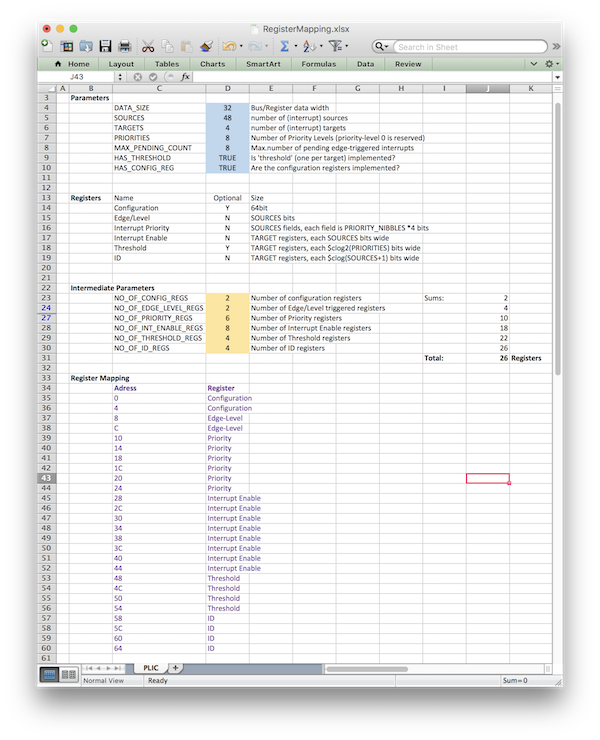
\includegraphics{../assets/graphics/AHB-Lite_PLIC_Worksheet.png}
\caption{Register Mapping Worksheet}
\label{fig:WORKSHEET}
\end{figure}

